\chapter{Lösungsstrategie von InstantAmbient}
Nachdem im letzten Kapitel ausführlich der Aufbau und die Verarbeitung von Konfigurationen diskutiert wurde, widmet sich dieses den verarbeitenden Systemen.
Lösungsstrategien bedeutet, dass ein Überblick darüber gegeben wird wie im generellen konfigurationsbasierte Dienste aufgebaut sein können.

\section{Anforderungen}
Ein sehr wichtiger Bestandteil den InstantAmbient erfüllen muss ist die Skalierbarkeit. Das System muss in einer kleineren Umgebung wie dem Auto als auch in einer großen Umgebung wie einem Hotel funktionieren. Demzufolge muss das System auch eine sehr große Last aushalten können. Hier ist die Last auf Grund der hohen Anzahl an verschiedene Räume ein ausschlaggebender Punkt. Es muss also möglich sein, dass mehrere Leute zur gleichen Zeit ihre Konfiguration senden können und diese dann ohne Probleme vom System verarbeitet werden. Des Weiteren muss das System eine verständliche Benutzerführung haben. Dementsprechend muss der Client eine sehr leicht zu bedienende Oberfläche mit kurzen Wegen haben. Dies erleichtert dem Benutzer das leichte und schnelle ändern von Konfigurationen.   

\section{Backend orientiert}
Um einen konfigurationsbasierten Dienst zu realisieren stehen verschieden Richtungen in denen man das System entwerfen kann. 
Zum einen besteht die Möglichkeit, die gesamten Daten im Backend\footnote{Oder auch der Cloud.} zu lagern. Zum anderen gibt es die Möglichkeit, die gesamten Daten auf dem Client zu Speichern. Dieses wird im nächsten Abschnitt näher erläutert.
\\\\
Entwickelt man das System Backend lästig bedeutet dies, dass die gesamten Daten von InstantAmbient im Backend persistiert werden. 
\\\\
Dadurch wird auch eine Benutzerverwaltung benötigt. Ohne diese wäre es nicht möglich die Konfigurationsdaten zu dem jeweiligen Benutzer möglich zuzuordnen. Damit der Benutzer selber seine Konfiguration vornehmen kann, benötigt das Backend eine Benutzerschnittstelle. Dabei gibt es verschiedene Möglichkeiten. Man könnte im Bereich von Hotels und Autovermietungen ein Terminal bereitstellen bei dem sich der Benutzer anmeldet um seine Umgebung auf seine Wünsche anzupassen. Dies führt mit sich, dass das Terminal an einem leicht zu erreichenden Standort steht. Eine andere Möglichkeit ist die Verwaltung mittels eines Webclients. Bei der Autovermietung sowie bei Hotels ist es für den Benutzer nicht unbedingt komfortabel sich erst noch an ein Terminal zu stellen um seine gewünschte Änderungen vorzunehmen. Die zentrale Sammlung der Daten bring Vor- sowie Nachteile, so ist eine Datenanalyse über den kompletten Bestand ein leichtes, dennoch muss eine entsprechende Sicherung dieser vorgenommen werden. 
\begin{figure}[H]
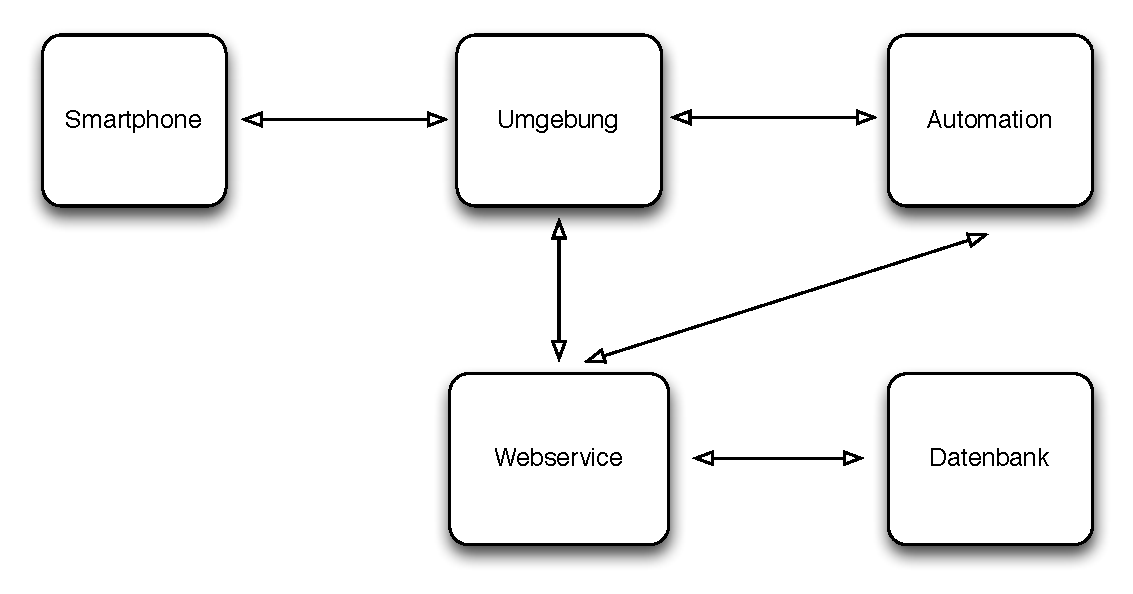
\includegraphics[width=12.5cm]{images/backend}
\caption{Konzept eines Backend orientierten Systems}
\end{figure}

Ein weiterer Aspekt ist die Authentifizierung. Bei der selbstständigen Benutzerverwaltung kann dies sehr einfach mit einem Benutzernamen und einen Passwort erfolgen, allerdings ist die bei der Authentifizierung im Auto oder Hotelzimmer zum Laden der Daten nicht unbedingt Benutzerfreundlich. Hierbei könnte man natürlich auf Smartcards oder RFID-Tags in Form eines runden Schlüsselanhänger zurückgreifen. Dieser würde dann nur zu Authentifizierung dienen, wodurch das System weiß, welches Profil geladen und an die Umgebung geschickt werden muss. Zusätzlich gibt es hierbei noch die Möglichkeit das System zentral oder dezentral aufzubauen. Das bedeutet wiederum, dass die Daten an die jeweilige Umgebung überführt werden müssen und das Diese einen großen Datenspeicher brauchen, da eine Vielzahl von Personen die Umgebung nutzen, wie bei einer Vermietung oder einem Hotel. Natürlich können auch nur die Daten in der Umgebung gespeichert werden, von den Personen die sich in der nächsten Zeit in dieser Umgebung befinden. Allerdings haben die Benutzer dann nicht die aktuelle Konfiguration ihrer Umgebung, falls diese am bereitgestellten Terminal noch Änderungen vornehmen.  

\section{Client orientiert}

Wie schon angesprochen, ist bei einem Client orientiertem System gemeint, dass die Daten auf diesem Gerät gespeichert werden, wodurch der Client an Umfang und Komplexität zunimmt. Auf Grund der einfachen Handhabung und der Datenmenge, die bei einem solchen System auf dem Client gespeichert wird, ist in diesem Fall ein Smartphone als Client am praktikabelsten.  
\\\\
Durch die Verfügbarkeit eines Smartphone als Client hat man die Möglichkeit eine App zu entwickeln, die es dem/der BenutzerIn ermöglicht seine Umgebung jederzeit zu konfigurieren und auf dem Gerät zu speichern. Würde man auf eine Alternative wie zum Beispiel eine Smartcard setzten bräuchte man hierfür wiederum ein Lese- und Schreibgerät sowie eine Anwendung um seine Umgebung zu Konfigurieren und auf die Smartcard zu übertragen. Dies ist ein weiterer Aspekt der für das Smartphone spricht.
\\\\
Durch die Verwendung eines externen Datenspeichers müssen die Daten nicht mehr im Backend gespeichert werden, wodurch keine große Speicherkapazität mehr benötigt wird. Es wird auch keine Schnittstelle wie ein Terminal oder ein Webclient benötigt. Da in diesem Fall der Datenspeicher Personengebunden ist, ist auch keine Benutzerverwaltung mehr notwendig. Somit bekommt das Backend eine Fokussierung auf das Empfangen und die Verarbeitung der Konfiguration sowie das Ansprechen der richtigen Umgebung.
Da bei einem Client orientierten System die gesammelten Konfigurationen, von allen Umgebungen die eine Person angelegt hat, auf dem Client vorhanden ist, muss dieser darüber informiert werden welche Konfiguration er gerade senden soll. 
\begin{figure}[H]
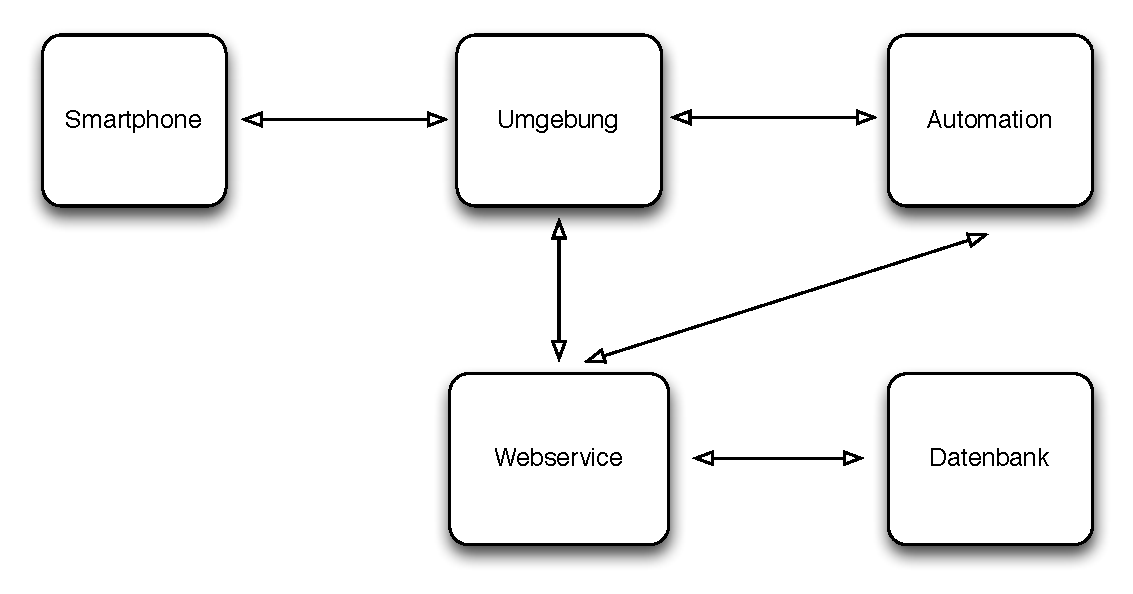
\includegraphics[width=12.5cm]{images/client}
\caption{Ein Client orientiertes System}
\end{figure}
Natürlich muss in diesem Fall das Backend dem Client darüber Informieren welche Konfiguration benötigt wird, damit der Client diese übertragen kann. Im Allgemeinen ist zu sagen das dieses System zwei ausgeglichene Seiten schafft. Zum einen die Clientseite, die zur Konfiguration der Daten und zur Speicherung dieser dient. Zum anderen die Backendseite, die zur Verarbeitung und ansprechen der jeweiligen Umgebungen dient. Ein Punkt den dieses System noch bietet ist, dass man durch das schlanke Backend dieses in beliebige Umgebungen einbauen kann und somit das System keinen Prinzipiellen unterschied zwischen einem Auto und einem Haus macht. Lediglich die Konfigurationsmöglichkeiten sowie die anzusprechenden Geräte sind unterschiedlich. Das bedeutet das Leichte austauschen von Komponenten.

\section{Proof of Concept}
Beim Vergleich dieser beiden Systeme kann man feststellen, dass das Prinzip eines Client orientierten Systems mehr Vorteile mit sich bringt. Da hierbei keine Terminals oder Speicherkapazität, zusätzlich zum Ansprechen der Aktoren benötigt wird. 
\\\\ 
Daher verfolgt InstantAmbient die Lösung dieses Systems. \\
Soviel vorweggenommen, als Client wird eine App für ein Android-Smartphone entwickelt. Dieser soll es dem/der BenutzerIn ermöglichen auf einfachen Weg Konfigurationen zu erstellen, zu bearbeiten und zu Speichern. Der Client soll sich dann über Bluetooth mit dem Backend verbinden und die Konfigurationen als JSON-Objekt an das Backend übertragen. Das Backend hat die Aufgabe die Daten zu empfangen, diese zu verarbeiten und dementsprechend die aufbereiteten Informationen an die jeweilige Schnittstelle der zu Konfigurierenden Geräte zu senden. 
Somit wird ein System entstehen in dem der/die BenutzerIn seine Daten Ortsunabhängig ändern kann und bei Verbindung des Clients mit dem Backend diese übertragen werden. 
\\\\
Im nächsten Kapitel wird die Architektur, Technologie und der Aufbau der einzelnen Komponenten genauer beleuchtet.
